\documentclass[class=article, crop=false]{standalone}

\usepackage{./resources/style}
\usepackage{./resources/referencing}

 \title{(10) Complex Integrals}
\date{Analysis (200023)}
\author{Analysis (200023)}
% \usepackage{cancel}
% \usepackage{geometry}
% \geometry{a4paper, portrait, margin=1in}
% \usepackage{centernot}
% \usepackage{wrapfig}
% \usepackage{amsmath}
% \usepackage{esint}
% \usepackage{steinmetz}
% \usepackage{lipsum}% http://ctan.org/pkg/lipsum
% \usepackage{amssymb}
% \usepackage{lmodern}
% \usepackage{graphicx}
% \usepackage{amsfonts}
% \usepackage{xfrac}
% %%Bookmarks does the PDF outline and \tableofcontents
% \usepackage[colorlinks=true,linkcolor=blue,urlcolor=black,bookmarksopen=true]{hyperref}
% \usepackage[depth=5]{bookmark}% Show up to level 4 (\paragraph) in bookmarks
% \setcounter{tocdepth}{3}% Show up to level 3 (\subsubsection) in ToC
% \usepackage{titlesec} %This is to stop the automatic numbering of sections (you can't use * with TOC)
% \usepackage[most]{tcolorbox} %Theorem Boxes
% \titleformat{\chapter}[display] %No Numbering for chapter
%   {\normalfont\bfseries}{}{0pt}{\Huge}
%
% %%Fix Headers Otherwise it has half an erroneous number in there
% \usepackage{fancyhdr}
% \pagestyle{fancy}
% %\fancyhf{}
% %\fancyhead[R]{\leftmark}
% %\fancyhead[L]{\rightmark}
% %\renewcommand\headrulewidth{0pt}
% %\renewcommand\chaptermark[1]{\markboth{#1}{}}
% %\renewcommand\sectionmark[1]{\markright{\thesection.\ #1}}
% \rhead[\rightmark]{\rightmark}
% \lhead[(8) Integrals]{(8) Integrals}
% %\fancyhead[R]{\rightmark}
%
% %%Stop Numbers for Sections
%
% \renewcommand{\thesection}{\hspace*{-1.0em}}
% \renewcommand{\thesubsection}{}
% \renewcommand{\thechapter}{}
% \renewcommand{\theequation}{\arabic{equation}}
%
% %% Get rid of the heading for the TOC
%
% \newtcbtheorem{Theorem}{Theorem}{
%   enhanced,
%   sharp corners,
%   attach boxed title to top left={
%     yshifttext=-1mm
%   },
%   colback=white,
%   colframe=blue!75!black,
%   fonttitle=\bfseries,
%   boxed title style={
%     sharp corners,
%     size=small,
%     colback=blue!75!black,
%     colframe=blue!75!black,
%   }
% }{thm}
% \newtcbtheorem[no counter]{Proof}{Proof}{
%   enhanced,
%   sharp corners,
%   attach boxed title to top left={
%     yshifttext=-1mm
%   },
%   colback=white,
%   colframe=blue!25,
%   fonttitle=\bfseries,
%   coltitle=black,
%   boxed title style={
%     sharp corners,
%     size=small,
%     colback=blue!25,
%     colframe=blue!25,
%   }
% }{prf}

\title{(10) Integrals}
\author{Analysis (200023)}


\begin{document}
	\maketitle
	\tableofcontents
	
        \section{Integrals from a Real Domain}
        To begin this consider the function:
        \[
        w: \mathbb{R}     \rightarrow \mathbb{C}  
        \]
        we can decompose such a function into real and imaginary components:
        \[
          w \left( t \right) =  u \left( t \right) +  i \cdot  v \left( t \right) 
        \]
        where $u$ and $v$ are purely real functions.
        \subsection{Differentiation}
        If $w =  f \left( z \right) $:
        \[
          f' \left( z \right) = \frac{\operatorname{d}w }{\operatorname{d} z} \quad \text{(As if $z$ was a purely real operator)}
        \]
        If $g\left( x,y \right)  =  u\left(  x,y  \right)  +  i \cdot  v \left( x, y \right) $: 

        \begin{align*}
        f'\left( z \right) &= \frac{\partial u }{\partial x}+ \frac{\partial v }{\partial x} \\
        &= \frac{dw}{dz}
        \end{align*}

        If $w =  u\left( t \right) + i \cdot v \left( t \right) $:
        \[
        w'\left( t \right) =  \frac{\operatorname{d}u }{\operatorname{d} t} + i \cdot \frac{\operatorname{d} v}{\operatorname{d} t}
        \]

        \subsection{Integration}
        If $w =  u\left( t \right) + i \cdot v \left( t \right) $:


        \[
        \int^{b}_{a}\left( w \left( t \right)  \right) \operatorname{d}t =  \int^{b}_{a}\left( u \right) \operatorname{d}t + i \cdot  \int^{ b}_{a}\left( v \right) \operatorname{d}t   
        \]

        \paragraph{Fundamental Theorem of Calculus} \ \\
        The fundamental theorem of calculus applies here:
        \begin{align}
         \int^{b}_{a}\left( w\left( t \right)  \right) \operatorname{d}t =  \left[ W\left( t \right)  \right]^b_a 
          \label{ftcest}
        \end{align}
        \subparagraph{Justification}

        let $W\left( t \right) =  U\left( t \right) +  i \cdot  V\left( t \right) $ be the antiderivative of $w\left( t \right) $:

        \begin{align*}
          \int^{b}_{a}\left( w \left( t \right)  \right) \operatorname{d}t &= \left[ U\left( t \right)  \right]^b_a + i\cdot \left[ v\left( t \right)  \right]^b_a \\
          &= \left[ U\left( b \right) + i\cdot V\left( b \right)  \right] -\left[ U\left( a \right) +  i \cdot V\left( a \right)  \right]  \\
          &= \left[ W\left( b \right) - W\left( a \right)  \right] \\
          &= \left[ W\left( t \right)  \right]^b_a
        \end{align*}
        \begin{flushright}
        {\rule{0.7em}{0.7em}}
        \end{flushright}
         
        \section{Contours}
        Integrals of complex valued functions are of the form:
        \[
          \lim_{n     \rightarrow \infty}\left( \sum^{n}_{i= 1}\left[ f\left( z^*_i \right) \cdot \Delta z \right]  \right)
        \]
         $\Delta z$ could be along any curve in the complex plane rather than just the axis along which we would integrate:
        
\begin{figure}[h!]
	
	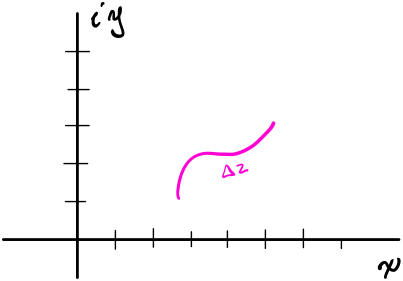
\includegraphics[width=0.3\linewidth]{./media/CompexIntegrals/handwriting.png}



	\label{fig:handwriting}
\end{figure}

this short curve is what we call a contour, the complex integral will be a line integral along that curve:


\begin{figure}[h!]
	\centering
	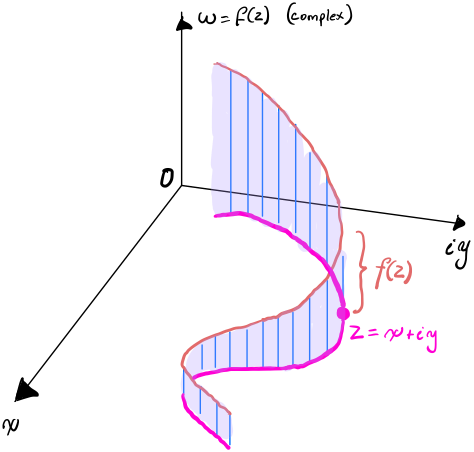
\includegraphics[width=0.3\linewidth]{"./media/CompexIntegrals/handwriting2.png"}
	\caption{}
	\label{fig:handwriting-2}
\end{figure}


\newpage


\paragraph{Define Contours}\ \\
A set of points $z =  \left( x,y \right)$ in the complex plane is said to be an \textbf{\textit{arc}} or a curve that we will call $C$ if:

\begin{align}
 x =  x\left( t \right), \quad y =  y\left( t \right) \qquad \left( a \leq t \leq b \right)
  \label{arcdef}
\end{align}

where:
\begin{itemize}
  \item $x\left( t \right)$ and $y\left( t \right) $ are continuous functions 
    \subitem continuous however does not mean smooth/differentiable, sharp points are allowed.
  \item the output values are ordered corresponding to $t$ (as if $t$ represented time)
\end{itemize}

It is more convenient to describe the curve at (\ref{arcdef}) as:

\begin{align}
  z &= z\left( t \right)  \label{arccompdef} \\
  &= x\left( t \right) + i\cdot y\left( t \right) \notag
\end{align}

\subparagraph{Types of Arcs}\ \\
\begin{itemize}
  \item A \textbf{Simple Curve} does not cross itself
  \item a \textbf{Closed Curve} meets back up with itself
  \item a \textbf{Simple Closed Curve} is closed and does not cross itself (except where it closes)
  \item a \textbf{Positive Curve} moves counter-clockwise as $t$ increases.
\end{itemize}
\begin{figure}[h!]
	
	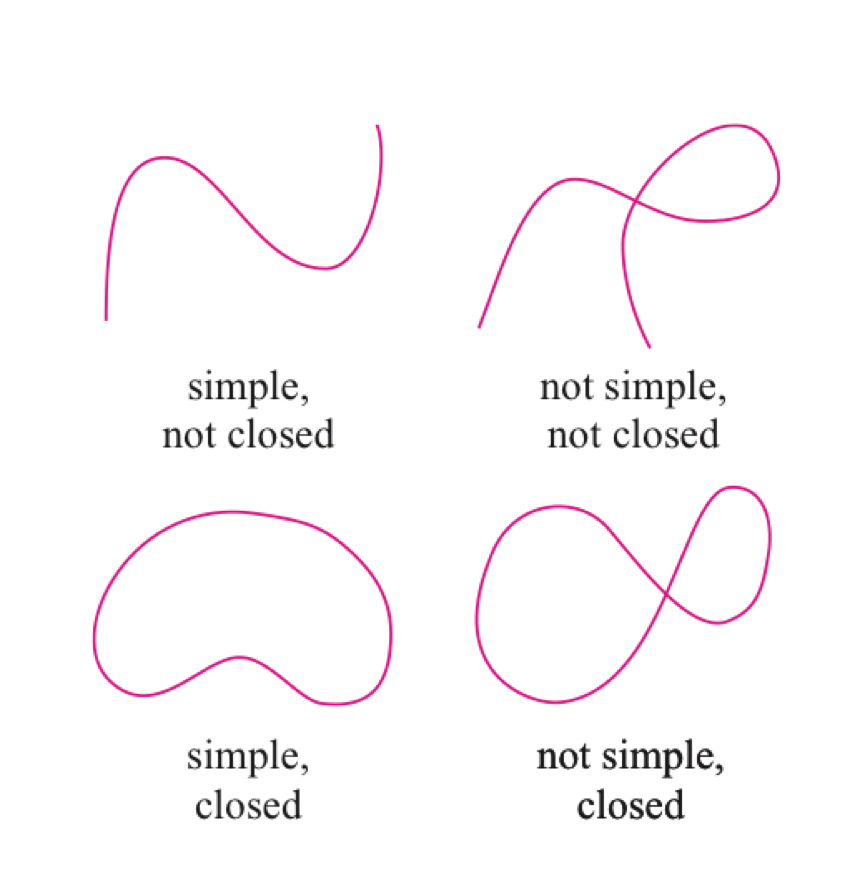
\includegraphics[width=0.2\linewidth]{"./media/CompexIntegrals/Image.png"}

	\label{fig:image}
\end{figure}

\subparagraph{Parametric Representation not unique}\ \\
Also the parametric representation of such a curve is not unique, the same curve could be represented by lots of different parametric equations, just like a second degree polynomial can also be modelled by a 3rd degree polynomial between intervals.

\newpage


\section{Contour Integral}
As previously discussed, an integral with respect to $z$ will be a contour integral:
\[
\int^{}_{C} f \left(z \right)   \operatorname{d}z 
\]
If the value of the integral does not depend on the path of the contour and only depends on the endpoints then we would write:

\[
\int^{}_{C} f \left(z \right)   \operatorname{d}z = \int^{z_2}_{z_1} f\left( z   \right) \operatorname{d}z 
\]
We can also put the integral in terms of the contour parameters, This is basically \textit{Integration by Substitution} in reverse, there's a more rigorous proof in the textbook by \textit{Osbourne}, just take it as definition.

  \begin{align}
    \int^{}_{C}\left( f\left( z \right)  \right) \operatorname{d}z = \int^{b}_{a}\left(f \left[ z\left( t \right)  \right]\cdot  z'\left( t \right)  \right) \operatorname{d}t  
    \label{tdef}
  \end{align}
  
\paragraph{Negative Contours}\ \\
If a contour $C$ is given the contour $- C$ denotes the same contour with the order of the points reversed.
Hence we have:

\begin{align*}
\int^{}_{-C}\left( f\left( z \right)  \right) \operatorname{d}z  &= \int^{- a}_{- b}\left( f\left[ z\left( - t \right)  \right] \cdot \frac{\operatorname{d} }{\operatorname{d} t}\left( z\left( - t \right)  \right)  \right) \operatorname{d}t \\
    &= - \int^{b}_{a}\left( f\left[ z\left( - t \right)  \right] z'\left( - t \right)  \right) \operatorname{d}t \\
    &= - \int^{}_{C}\left( f\left( z \right)  \right) \operatorname{d}z 
\end{align*}


Refer to p. 128 of \textit{Churchill's 9th} for worked examples.

\subsection{Notation}
If we want to basically i want to know does the symbol:
\[
\oint^{}_{} f\left( z \right)   \operatorname{d}z
\]
\begin{itemize}
  \item a contour/line integral of any sort
  \item a contour/line integral around a closed path
  \item one of the above but specifically in the anticlockwise direction?
\end{itemize}

\subsection{Upper Bounds for Moduli}

Start with the triangle inequality:
\[
    \left| \alpha + \beta \right| \leq     \left| \alpha \right| +     \left| \beta \right| 
\]
We could prove this, or, by similar reasoning:

\begin{align*}
\implies      \left| \int^{}_{}\left( w\left(  t \right)  \right) \operatorname{d}t  \right| &\leq \int^{}_{} \left| w\left( t  \right|  \right) \operatorname{d}t 
\end{align*}

   Now let:
   \begin{itemize}
     \item $C$ be a contour of length $L$
     \item  $    \left| f\left( z \right)  \right| \leq M$
   \end{itemize}

   Using the inequality above it can be rigorously shown:

   \[
       \left| \int^{}_{}\left( f\left( z \right)  \right) \operatorname{d}z  \right| \leq M\cdot L
   \]

   This can be somewhat visualised if $f\left( z \right) $ is taken to be the height of the function along the contour, and $L$ is taken to be the length of the contour, although the values will be complex and height might become an odd concept, the mathematics should still hold.
   \paragraph{Example}
   Evaluate the contour integral:
   \[
     \int^{}_{C}\left( \frac{1}{z} \right) \operatorname{d}z 
   \]
   Where:
\begin{itemize}
     \item $C:     \left| z \right| = 1$
\end{itemize}

\noindent   Now put the integral in terms of the parametric representation (\ref{tdef}):

   \begin{align}
       \int^{}_{C}\left( \frac{1}{z} \right) \operatorname{d}z &=  \int^{\pi}_{\pi}\left( \frac{1}{e^{i\theta}} \cdot \frac{\operatorname{d} }{\operatorname{d} \theta}\left( e^{i\theta} \right)  \right) \operatorname{d}\theta \notag \\
       &= \int^{\pi}_{\pi}\left( \frac{1}{e^{i\theta}} \cdot i\cdot e^{i\theta} \right) \operatorname{d}\theta \notag \\
       &= \int^{\pi}_{\pi}\left( i \right) \operatorname{d}\theta \notag \\  
       &= \left[ i \cdot \theta \right]^{\pi}_{\pi} \notag \\
       &= 0
     \label{excontint1}
   \end{align}

   \section{Antiderivatives}
   Generally the value of a contour integral depends on both the path of the contour and the function.\\
   Some contour intergrals however have values independent of the path, for example consider how many integrals over closed paths will have an integral of zero as in the example above.\\

   The antiderivative of a complex function is $F\left( z \right) $ such that:
   \[
   F'\left( z \right) = f\left( z \right) 
   \]
   The antiderivative is, of necessity, an analytic function.

   The antiderivative is uniqe, there is only one antiderivative for a given funciton (other than the additive constant $\left( +  C \right) $ component).

   \subsection{Basic Antiderivative Theorem}
   Suppose $f\left( z \right) $ is continuous in a domain, if the function has an antiderivative $F\left( z \right) $ through the domain then:

   \ \
   
   \hfill\begin{minipage}{\dimexpr\textwidth-3cm}
   integrals of $f\left( z \right) $ along contours lying in the domain depend only on the endpoints of that contour:
   \[
     \int^{}_{C}f\left( z \right)  \operatorname{d}z = \int^{z_2}_{z_1} f\left( z \right)   \operatorname{d}z = \left[ F\left( z \right)  \right]^{z_2}_{z_1} 
   \]

   This also means that integrals around a closed contour will be 0.
   \end{minipage}
   \ \
   

   \paragraph{Proof}
   if $F'\left( z \right)  = f\left( z \right) $ :
   
   \begin{align*}
       \int^{}_{C} f\left( z \right)   \operatorname{d}z &=  \int^{b}_{a} f\left( z\left( t \right)  \right)   \operatorname{d}t \\
       &= \int^{b}_{a} U\left( z\left( t \right)  \right)   \operatorname{d}t + i\cdot \int^{b}_{a} b\left( z\left( t \right)  \right)   \operatorname{d}t\\
       \intertext{Which means the Fundamental Theorem of Calculus Applies from (\ref{ftcest})}
       &= F\left( z\left( b \right)  \right) - F\left( z\left( a \right)  \right) \\
       &=  F\left( z_2 \right) - F\left( z_1 \right) \\
       &= \left[ F\left( z \right)  \right]^{z_2}_{z_1} \\
       &= \left[ U\left( t \right)  \right]^{b}_{a} +  i \cdot  \left[ V\left( t \right)  \right]^{b}_{a} \\
       &= U\left( b \right) - U\left( a \right) +  i \cdot  \left[ V\left( b \right) - V\left( a \right)  \right] \\
       &= \left[ U\left( b \right)+  V\left( b   \right)  \right] -  i \cdot  \left[ U\left( a \right) - V\left( b \right)  \right] \\
       &= F\left( b \right) - F\left( a \right) \\
       &= \left[ F\left( z \right)  \right]^{b}_{a}\\
       &= \left[ F\left( z \right)  \right]^{z_2}_{z_1}
   \end{align*}

   \section{Cauchy Goursat Theorem}
   This theorem depends on \textit{Green's Theorem} which gives the relationship between a line integral around a simple-closed curve and the double integral over the corresponding bounded region, for purely real functions. Roughly Speaking \textit{Green's Theorem} is a counterpart of the Fundamental Theorem of Calculus for double integrals.\\

   In establishing the \textit{Cauchy-Goursat Theorem}, proving \textit{Green's Theorem} is the tricky part, the \textit{Cauchy-Goursat Theorem}  more or less falls out of it. 

\ \

\hfill\begin{minipage}{\dimexpr\textwidth-3cm}
\begin{tcolorbox}

  \subparagraph{ the \textit{Cauchy-Goursat Theorem}} 

  If a function $f$ is analytic at all points interior to, and on, a simple closed contour $C$, then:

  \[
  \oint^{}_{C} f\left( z \right)   \operatorname{d}z = 0 
  \]
\end{tcolorbox}

\end{minipage}
\ \

\subsection{Simply-Connected Domains}
If $f\left( z \right) $ is analytic through a simply connected domain:
\[
\int^{}_{C} f\left( z \right)   \operatorname{d}z 
\]
Where:
\begin{itemize}
  \item C is any closed contour in that domain (Simple or not)
    \subitem i.e. if the domain is simply connected, the contour can cross itself.
\end{itemize}

From this it follows:
\begin{itemize}
  \item If a function is analytic on a simply connected domain, then:
    \subitem there will be an anti-derivative:
    \subsubitem The contour integral will be independent of path (i.e.$F(b) - F(a)$ 
    \item Entire functions always have an antiderivative
      \subitem and will always be independent of path.
\end{itemize}

\subsection{Multiply Connected Domains}
If $C$ is a closed counter-clockwise contour, inside which are closed Clockwise contours $c_1, c_2, c_3 \dots$ for which the function is analytic interior to C but exterior to $c_1, c_2, c_3 \dots$ :


\begin{figure}[h!]
	\centering
	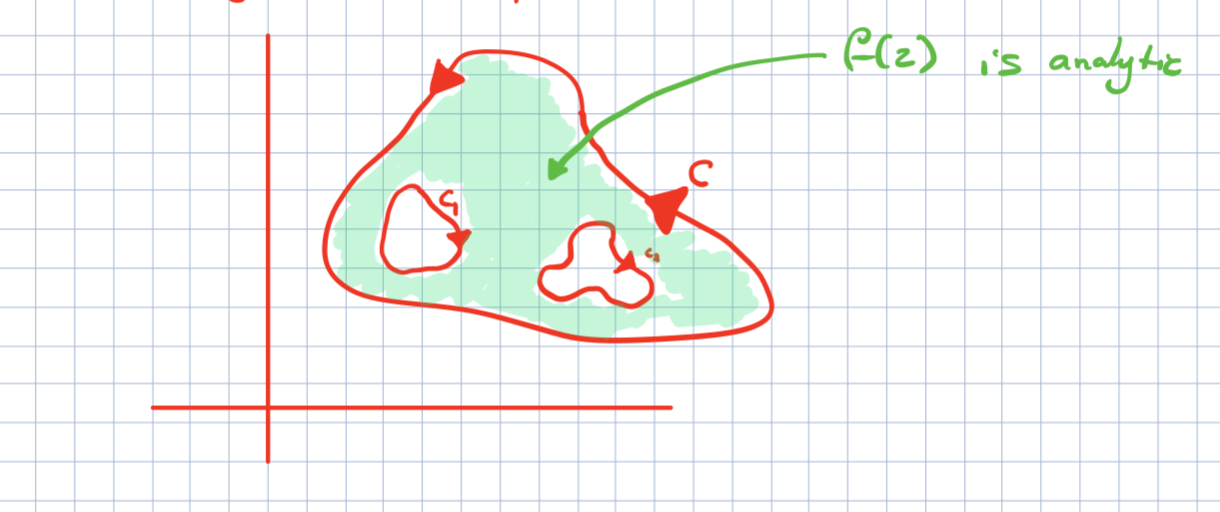
\includegraphics[width=0.7\linewidth]{./media/CompexIntegrals/s1.png}
	\caption{}
	\label{fig:s1}
\end{figure}



Then we have:

\[
\int^{}_{C} f\left( z \right)   \operatorname{d}z + \sum^{k}_{n= 1} \left[ \int^{}_{c_n} f\left( z \right)   \operatorname{d}z  \right] 
\]
This is established by drawing a line through all the interior closed contours and applying the \textit{Cauchy-Goursat} theorem, refer to the \textit{Churchill} textbook.

\paragraph{Principle of Deformation}
If we had Something like this:

\begin{figure}[h!]
	\centering
	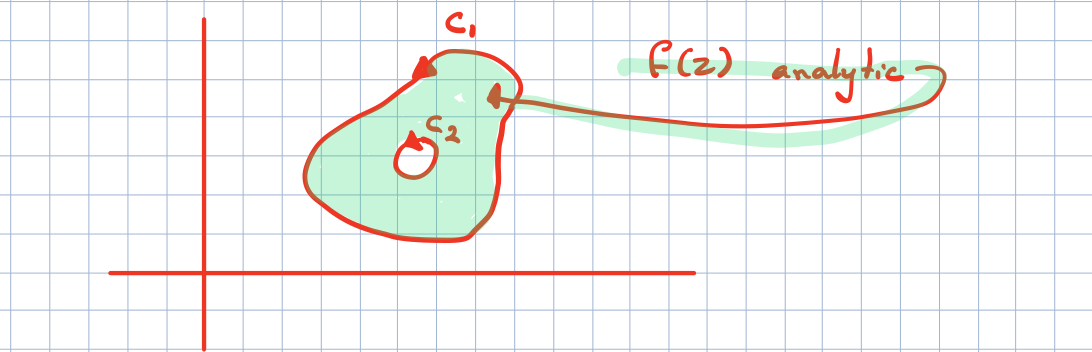
\includegraphics[width=0.7\linewidth]{./media/CompexIntegrals/s2.png}
	\caption{}
	\label{fig:s2}
\end{figure}


Then it would follow:

\begin{align*}
  \int^{}_{C_1} f\left( z \right)   \operatorname{d}z + \int^{}_{c_2} f\left( z \right)   \operatorname{d}z &= 0\\  
  \int^{}_{C_1} f\left( z \right)   \operatorname{d}z - \int^{}_{c_2} f\left( z \right)   \operatorname{d}z &= 0\\
  \int^{}_{C_1} f\left( z \right)   \operatorname{d}z &= \int^{}_{c_2} f\left( z \right)   \operatorname{d}z  
\end{align*}

So if $c_2$ can be continuously transformed into $C_1$ through an analytic region, then the integral is the same.

\subparagraph{Spacial Case of Deformation}
We Should Probably memorise this special case:

\[
\ointctrclockwise^{}_{    \left| z - z_0 \right| = r} \left( z- z_0 \right) ^n  \operatorname{d}z = 
\begin{cases}
  0 \qquad if n \neq - 1\\
  2\pi i \qquad if n = - 12
\end{cases}
\]

\subparagraph{Example}

\begin{align*}
    \int^{}_{    \left| z \right| = 1} \frac{1}{z^2 +  2z+2 }  \operatorname{d}z &= \int^{}_{    \left| z \right| = 1} \frac{1}{\left( z +  \left( 1 +  i \right)  \right) \cdot \left( z +  \left( 1 -  i \right)  \right) }  \operatorname{d}z  \\
    \intertext{There is a singularity at $z =  - 1 \pm i$, which is outside the closed countour, the function is analytic everwhere else inside and on the closed countour hence by the \textit{Cauchy-Goursatt Theorem:}}\\
  \int^{}_{    \left| z \right| = 1} \frac{1}{z^2 +  2z +  2}  \operatorname{d}z &= 0 
\end{align*}

\section{Cauchy Integral Formula}
This has to be memorised.\ \\

\hfill\begin{minipage}{\dimexpr\textwidth-3cm}
\begin{tcolorbox}

  \subparagraph{Cauchy Integral Formula}\ \\
If $f$ is analytic everwhere inside and on $C$ and $z_0$ is interior to C:
\[
  \int^{}_{C} \frac{f\left( z \right) }{z - z_0}  \operatorname{d}z = 2\pi i \cdot  f \left( z_0 \right)  
\]
\end{tcolorbox}

\end{minipage}
\ \


\paragraph{Example}
Solve :
\[
\int^{}_{    \left| z \right| = 1} \frac{\cos{z}}{z^3 +  9z}   \operatorname{d}z 
\]
First simplify the intergrand somewhat:

\[
  \int^{}_{    \left| z \right| = 1} \frac{\cos{z}}{z^3 +  9z}  \operatorname{d}z = \int^{}_{    \left| z \right| = 1} \frac{1}{z} \cdot  \frac{\cos{z}}{z^2 +  9z}  \operatorname{d}z  
\]


Observe that the intergrand $\frac{\cos{z}}{z^3 +  9z}$ is analytic everywhere other than its singularities:

\begin{itemize}
  \item $z =  0$ 
  \item $z = 3i$
  \item $z =  - 3i$ 
\end{itemize}


because $z = 0$ is inside the contour we cannot use the \textit{Cauchy-Goursatt Theorem}, however, we can use the \textit{Cauchy-Integral Formula} precisely because :
\begin{itemize}
  \item $z_0 = 0$ is interior to the closed contour
  \item $f\left( z \right) = \frac{\cos{z}}{z^2+ 9} $ is analytic everywhere else interior to the closed contour
\end{itemize}

So by the Cauchy Integral Formula:

\begin{align*}
    \int^{}_{    \left| z \right| = 1} \frac{\frac{\cos{z}}{z^2+ 9}}{\left( z- 0 \right) }  \operatorname{d}z &= 2\pi i \cdot \frac{\cos{\left( 0 \right) }}{0^2+ 9} \\
    &= i\cdot \frac{2\pi}{9}
\end{align*}

\section{Extension of the Cauchy Integral Formula}
This has to be memorised:

 \ \

\hfill\begin{minipage}{\dimexpr\textwidth-3cm}
\begin{tcolorbox}
  \subparagraph{Extension to Cauchy Integral}\ \\

if:
\begin{itemize}
  \item $f\left( z \right) $ is analytic on and interior to some closed contour $C$ 
  \item $z_0$ is interior to $C$ 
\end{itemize}

Then:
\[
  \int^{}_{C} \frac{f\left( z \right) }{\left( z- z_0 \right) ^{n+ 1}}  \operatorname{d}z = f^{n}\left( z_0 \right) \cdot \frac{2\pi i}{n!} 
\]
\end{tcolorbox}

\end{minipage}
\ \




\end{document}
